\documentclass{article}
\thispagestyle{empty}

%Laden externer Dateien
\usepackage{import}
%Laden der Package-Konfigurationen
\import{../../../Documents/Latex/Preamble/}{pre_packages.tex}
%Lade die Klasse script
%\loadclass{script}

\usepackage{listings}

%Definiere Counter /numctr zur Nummerierung von equations
\newcounter{numctr}
%Füge /section in die Reset-Liste von /numctr hinzu
\makeatletter
\@addtoreset{numctr}{section}
\makeatother

%Math-Umgebungen werden umbrechbar
\allowdisplaybreaks

\pgfplotsset{compat=1.16}

\def\I{\mathbb}


% plotting
\usepackage{pgf,tikz,pgfplots}
\usepackage{mathrsfs}
\usetikzlibrary{arrows}

\usepackage{tikz-cd} 
\usepackage{xcolor}
\usepackage{svg}



\begin{document}

\pagestyle{plain}
\begin{tabular}{c c c c}

\begin{tikzpicture}[line cap=round,line join=round,>=triangle 45,x=1cm,y=1cm]
\draw (0,0) -- (1,0) -- (1,1) -- (0,1) -- (0,0); 
\end{tikzpicture} &
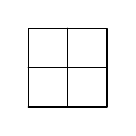
\begin{tikzpicture}[line cap=round,line join=round,>=triangle 45,x=1cm,y=1cm]
\draw (0,0) -- (1,0) -- (1,1) -- (0,1) -- (0,0);
{\color{black}
\draw (0,0.5) -- (1,0.5);
\draw (0.5,0) -- (0.5,1);
}
\end{tikzpicture}  & 
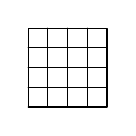
\begin{tikzpicture}[line cap=round,line join=round,>=triangle 45,x=1cm,y=1cm]
\draw (0,0) -- (1,0) -- (1,1) -- (0,1) -- (0,0);
\draw (0,0.5) -- (1,0.5);
\draw (0.5,0) -- (0.5,1);
{\color{black}
\draw (0,0.25) -- (1,0.25);
\draw (0,0.75) -- (1,0.75);
\draw (0.25,0) -- (0.25,1);
\draw (0.75,0) -- (0.75,1);
}
\end{tikzpicture} &
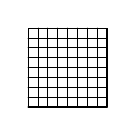
\begin{tikzpicture}[line cap=round,line join=round,>=triangle 45,x=1cm,y=1cm]
\draw (0,0) -- (1,0) -- (1,1) -- (0,1) -- (0,0);
\draw (0,0) -- (1,0) -- (1,1) -- (0,1) -- (0,0);
\draw (0,0.5) -- (1,0.5);
\draw (0.5,0) -- (0.5,1);
\draw (0,0.25) -- (1,0.25);
\draw (0,0.75) -- (1,0.75);
\draw (0.25,0) -- (0.25,1);
\draw (0.75,0) -- (0.75,1);
{\color{black}
\draw (0,0.125) -- (1,0.125);
\draw (0,0.375) -- (1,0.375);
\draw (0,0.625) -- (1,0.625);
\draw (0,0.875) -- (1,0.875);
\draw (0.125,0) -- (0.125,1);
\draw (0.375,0) -- (0.375,1);
\draw (0.625,0) -- (0.625,1);
\draw (0.875,0) -- (0.875,1);
}
\end{tikzpicture}

\end{tabular}

\end{document}